\chapter{Analyse / Fit}
Um aus einem Datensatz den \glqq wahren\grqq Wert diverser Parameter abzuschätzen, gibt es verschiedene Möglichkeiten. In dieser Analyse wird die Methode sFit verwendet. Diese stellt eine modifizierte Variante des \glqq Unbinned Maximum Likelihood\grqq Fits dar. Unbinned meint, dass das Fitergebnis nicht von der Wahl der Säulen (engl. bins) eines Histogramms abhängt. Die Modifikation des Fits besteht in der Verwendung der aus der \SPlot-Technik bekannten sWeights. Dadurch ist es nicht nötig, den Untergrund zu modellieren, da dieser aus statistischen Gründen annihiliert wird.

\section{Maximum Likelihood Funktion}
Die Maximum Likelihood Methode ist eine weit verbreite Methode, um Parameter abzuschätzen. Für eine gegebene Wahrscheinlichkeitsdichtefunktion (WDF) $\mathcal{P}(\vec{x_e};\vec{\lambda})$ mit einem unbekannten Satz Parametern $\vec{\lambda}$ und $N$ unabhängigen Messungen $\vec{x_e}$ ist die Likelihood-Funktion als
\begin{align}
\mathcal{L}(\vec{\lambda}) = \prod_{i=1}^N \mathcal{P}(\vec{x_e};\vec{\lambda})
\end{align}
definiert. Der Satz an Parametern, der $\mathcal{L}$ maximiert, gilt als beste Abschätzung von $\vec{\lambda}$. In der Praxis jedoch minimiert man äquivalent $-\ln\mathcal{L}$. Gewöhnlicherweise berücksichtigt man möglichen Untergrund, indem man die WDF in einen Signal- und Untergrundanteil aufteilt:
\begin{align}
\mathcal{P}(\vec{x_e};\vec{\lambda}) = f_{sig}\mathcal{P}_{sig}(\vec{x_e};\vec{\lambda}) + (1-f_{sig})\mathcal{P}_{bkg}(\vec{x_e}). \label{eq:likelihood_sig_bkg}
\end{align}
$f_{sig}$ bezeichnet hierbei den Signalanteil, $\mathcal{P}_{sig}, \mathcal{P}_{bkg}$ die WDF des Signals bzw. Untergunds. Die Schwierigkeit besteht nun darin, den Untergrund geeignet zu modellieren. Dazu bedarf es MonteCarlo-Studien oder der Verwendung separater Seitenbänder. \cite{sfit}

\section{Fitmethode sFit} \label{kap:sfit}
Der sFit bietet nun eine Möglichkeit, ohne genaue Kenntnis des Hintergrunds die wahre Verteilung des Signalanteils von $\vec{x}$ zu rekonstruieren. Dazu bedarf es einer weiteren Variable $\vec{y}$, die vollkommen unkorreliert ist, also sowohl für Signal als auch Untergrund. In dieser Analyse wird später $\vec{y} = y = M($\Bd$)$ die rekonstruierte Masse der \Bd sein, $\vec{x}^T = (t,d,\eta)^T$, die Variablen, die zur Bestimmung von $\SJPsi$ notwendig sind. Was diese im Einzelnen bedeuten wird später behandelt.

Sei $N_s$ die Zahl an Signal- und $N_b$ die Zahl an Untergrund-Ereignissen eines Datensatzes. Die Verteilungen von Signal und Untergund seien mit $F_s(y)$ bzw. $F_b(y)$ bezeichnet und all diese vier Größen seien bekannt. Dann stellt die \SPlot-Technik (\cite{splot}) mit den sogenannten \glqq sWeights\grqq 
\begin{align}
W_s(y) = \frac{V_{ss}F_s(y)+V_{sb}F_b(y)}{N_sF_s(y)+N_bF_b(y)}
\end{align} 
einen Formalismus zur Verfügung, um durch Gewichtung der Ereignisse Signal vom Untergrund zu bereinigen. Die Matrix $V_{ij}$ bezeichnet dabei das Inverse der Kovarianzmatrix
\begin{align}
V_{ij}^{-1} = \sum_{e=1}^N \frac{F_i(y_e)F_j(y_e)}{(N_sF_s(y_e)+N_bF_b(y_e))^2}.
\end{align}
In der \SPlot-Technik werden die Gewichte $W_s(y_e)$ berechnet und anschließend ein Histogramm mit den Messungen $x_e$ mit der entsprechenden Gewichtung gefüllt, um die wahre Verteilung von x zu erhalten. Beim sFit wird nun die Likelihood Funktion gemäß
\begin{align}
\mathcal{L}_W(\vec{\lambda}) = \prod_{i=1}^N \mathcal{P}(\vec{x_e};\vec{\lambda})^{W_s(y_e)}
\end{align}
gewichtet. Die Erwartung ist, dass der Untergrundanteil auf statistischer Grundlage eliminiert wird und der wahren Wert von $\vec{\lambda}$ durch Maximierung von $\mathcal{L}_W(\vec{\lambda})$ abgeschätzt werden kann.

\section{Bestimmung der sWeigths - Massenfit}
Wie bereits in Kapitel \ref{kap:sfit} erwähnt, wird die rekonstruierte Masse zur Berechnung der sWeights herangezogen. Dazu wird ein klassischer Maximum Likelihood durchgeführt, d.h. Signal und Untergrund werden gemäß Gleichung \ref{eq:likelihood_sig_bkg} gesondert beschrieben.

Für den Signalteil der Massenverteilung wird ein doppelter Gauß der Form
\begin{align}
\mathcal{P}_{m;S}(m;\vec{\lambda_{m;S}}) = f_{S,m}\mathcal{G}(m;m_{\text{\Bd}},\sigma_{m,1}) + \mathcal{G}(m;m_{\text{\Bd}},\sigma_{m,2})
\end{align}
mit gemeinsamen Mittelwert $m_{\text{\Bd}}$, unterschiedlichen Breiten $\sigma_{m,1}$ und $\sigma_{m,2}$ sowie dem relativen Beitrag $f_{S,m}$ der beiden Gauß-Kurven angenommen. Die Normierung ist dabei bereits in $\mathcal{G}$ enthalten.

Der Untergrund wird durch die Exponentialfunktion
\begin{align}
\mathcal{P}_{m;B}(m;\vec{\lambda_{m;B}}) = \frac{1}{\mathcal{N}_{m;B}}\e^{-\alpha_m m}
\end{align}
modelliert. $\mathcal{N}_{m;B}$ bezeichnet dabei die Normierung auf den im Fit verwendeten Massenbereich $m \in [5230,5330]\mega\electronvolt/c^2$. Damit lautet die gesamte Wahrscheinlichkeitsdichtefunktion der Massenverteilung
\begin{align}
\mathcal{P}_{m}(m;\vec{\lambda_{m}}) = f_{sig}\mathcal{P}_{m;S}(m;\vec{\lambda_{m;S}}) + (1-f_{sig})\mathcal{P}_{m;B}(m;\vec{\lambda_{m;B}}),
\end{align}
wobei $f_{sig}$ den Anteil des Signals angibt.

Der Fit liefert für den Parametersatz $\vec{\lambda_{m}}^T = (f_{sig}, f_{S,m}, m_{\text{\Bd}}, \sigma_{m,1},\sigma_{m,2}, \alpha_m)^T$ die in Tabelle \ref{tab:fit_masse} aufgeführten Resultate. Alle Parameter wurden dabei im Fit laufen gelassen. 

\begin{table}[hptb]
\centering
\caption{Ergebnisse des Massenfits zur Bestimmung der sWeights}
\label{tab:fit_masse}
$\begin{array}{lr@{\pm}ll}
\hline \hline
\text{Parameter} & \multicolumn{2}{c}{\text{Wert}} & \\ \hline
f_{sig}   & 0,676 & 0,047 &\\
f_{S,m}   & 0,804 & 0,050 &\\
m_{\text{\Bd}} & (5281,53 & 0,14)& \mega\electronvolt/c^2 \\
\sigma_{m,1} & (8,86 & 0,37)& \mega\electronvolt/c^2 \\
\sigma_{m,2} & (21,0 & 9,2) &\mega\electronvolt/c^2 \\
\alpha_m & (0,00158 & 0,00071) &(\mega\electronvolt/c^2)^{-1} \\ \hline
\end{array}$
\end{table}

Des Weiteren zeigt Abbildung \ref{fig:fit_masse} die Massenverteilung mit Fit, die dazugehörigen Pulls sowie die berechneten sWeights. Pulls sind die auf den Fehler des Messwerts normierten Residuen. Für eine beliebige Messgröße $y$ werden sie berechnet über
\begin{align}
pull(x) = \frac{y_{gemessen}-y_{gefittet}}{\sigma_y}.
\end{align}

\begin{figure}[hptb]
\centering
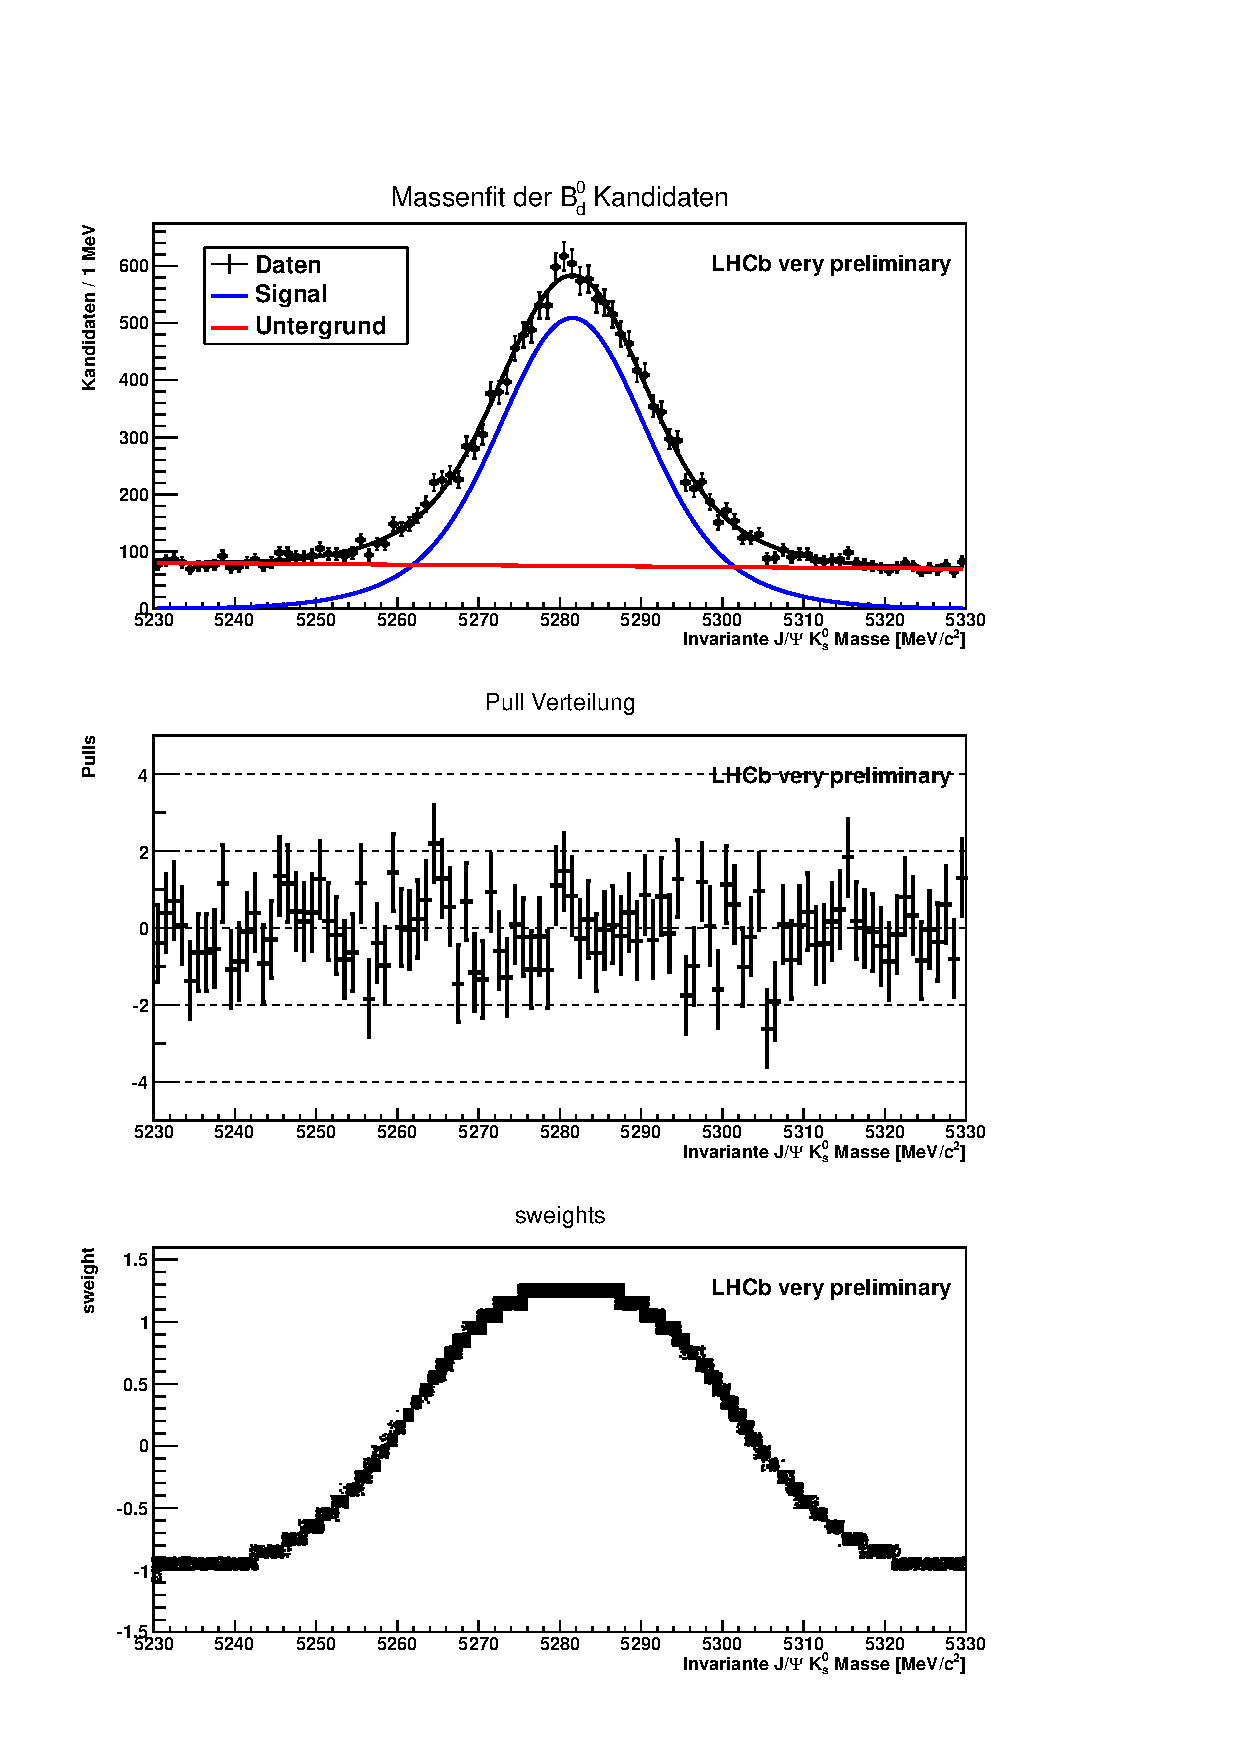
\includegraphics[width=\textwidth]{mass_fit}
\caption{Ergebnis des Massenfits}
\label{fig:fit_masse}
\end{figure}


\section{Wahrscheinlichkeitsdichtefunktion der Zerfallszeitverteilung}
In diesem Abschnitt soll nun die Wahrscheinlichkeitsdichtefunktion entwickelt werden, die letztendlich zur Bestimmung der Asymmetrie-Amplitude $\SJPsi$ verwendet wird. Aus den Gleichungen \ref{eq:bd} und \ref{eq:bdbar} geht für $|\lambda_f|=1$ die theoretische Zerfallszeitverteilung für ein \Bd bzw. \Bdbar hervor:
\begin{align}
\mathcal{P}_{\text{wahr}}(t, d_{\text{wahr}}) = \frac{1}{\mathcal{N}_t}\e^{-t/\tau}\left[1-d_{\text{wahr}}\SJPsi\sin(\sinarg)\right].
\end{align}
Durch die Einführung des wahren Tags $d_{\text{wahr}}$ wurden beide Verteilungen zu einer zusammengefasst. Ein anfängliches \Bd wird dabei durch $d_{\text{wahr}}=1$ beschrieben, ein \Bdbar durch $d_{\text{wahr}}=-1$. Die Normierung ist so gewählt, dass die Bedingung
\begin{align}
\sum_{d_{\text{wahr}}}\int_{t_{min}}^{t_{max}}\mathrm{d}t\mathcal{P}_{\text{wahr}}(t, d_{\text{wahr}}) = 1
\end{align}
erfüllt wird. Aufgrund zahlreicher detektorbedingten Effekte muss $\mathcal{P}_{\text{wahr}}(t, d_{\text{wahr}})$ modifiziert werden.

\subsection{Produktionsasymmetrie}
Der Detektor produziert \Bd- und \Bdbar-Mesonen nicht in exakt gleicher Zahl. Über die Produktionsraten $R_{\text{\Bdbar}}$ für ein \Bdbar bzw. $R_{\text{\Bd}}$ für ein \Bd ist die Produktionsasymmetrie definiert durch:
\begin{align}
\mu = A_P = \frac{R_{\text{\Bdbar}}-R_{\text{\Bd}}}{R_{\text{\Bdbar}}+R_{\text{\Bd}}}.
\end{align}
Anhand dieser Definition muss der Anteil an \Bd bzw. \Bdbar an der gesamten WDF gewichtet werden. Unter Verwendung des Kronecker-Deltas $\delta_{ij}$ lässt sich die WDF daher schreiben als:
\begin{align}
\nonumber \widetilde{\mathcal{P}}_{\text{wahr}}(t, d_{\text{wahr}}) &= \delta_{d_{\text{wahr}},1}(1-\mu)\mathcal{P}_{\text{wahr}}(t, 1) + \delta_{d_{\text{wahr}},-1}(1+\mu)\mathcal{P}_{\text{wahr}}(t, -1) \\
\nonumber &= (1-d_{\text{wahr}}\mu)\mathcal{P}_{\text{wahr}}(t, d_{\text{wahr}}) \\
&= \frac{1}{\mathcal{N}_t}\e^{-t/\tau}\left[1-d_{\text{wahr}}\mu - (d_{\text{wahr}}-\mu)\SJPsi\sin(\sinarg)\right].
\end{align}

\subsection{Bestimmung des Anfangszustandes der \Bd-Mesonen(Tagging)}
Die Messung der indirekten \CP-Verletzung setzt voraus, dass der anfängliche Flavour des \Bd-Mesons bekannt ist. Den Vorgang zu entscheiden, ob ein rekonstruierter Signalkandidat ein $b$ oder $\overline{b}$ Quark enthält, nennt man \glqq Flavour Tagging\grqq. Hierzu werden sogenannte Tagging Algorithmen angewandt, die allerdings keine perfekten Ergebnisse lieferen. Von $N$ Kandidaten kann bei $N_U$ Kanidaten kein Anfangsflavour zugeordnet werden, bei $N_W$ ist er falsch und bei $N_R$ ist er richtig. Ein Maß für die Güte des Algorithmus ist die Tagging Effizienz
\begin{align}
\epsilon_{\text{tag}} = \frac{N_R+N_W}{N_R+N_W+N_U}
\end{align}
und die Fehlerwahrscheinlichkeit
\begin{align}
\omega = \frac{N_W}{N_R+N_W},
\end{align}
die die Wahrscheinlichkeit angibt, den Signalkandidaten den falschen Flavour zuzuordnen. Die Größe die es bei solchen Algorithmen zu maximieren gilt, ist die effektive Tagging Effizienz
\begin{align}
\epsilon_{eff} = \epsilon_{tag}(1-2\omega)^2.
\end{align}

Bei dem in dieser Arbeit verwendeten Algorithmus handelt es sich um einen sog. Opposite Side Tagger (OST). Dieser nutzt aus, dass die meisten $b$ Quarks in Quark-Antiquark Paaren erzeugt werden. Dabei rekonstruiert der OST die Ladung der Zerfallsreste des entsprechenden Quark-Partners des \Bd-Mesons. Der Algorithmus berechnet aus kinematischen und geometrischen Daten eine Fehlerwahrscheinlichkeit $\eta^{OS} \in [0;0,5]$ für seine Flavour-Zuweisung (oder auch Tagging Entscheidung genannt), die im folgenden mit $d^{OS}$ bezeichnet wird. \cite{lhcb-paper}

Die vorhergesagte Fehlerwahrscheinlichkeit $\eta^{OS}$ muss allerdings noch auf diversen Zerfallskanälen kalibriert nehmen. Dies ist allerdings nicht Bestandteil dieser Arbeit, sondern wurde auch \cite{tagging} entnommen. Die Kalibrationsfunktion lautet:
\begin{align}
\omega(\eta^{OS}) = p_1\left(\eta^{OS}-\left\langle \eta^{OS} \right\rangle\right) + p_0 .
\end{align}
$\left\langle \eta^{OS} \right\rangle$ steht dabei für das arithmetische Mittel der $\eta^{OS}$-Verteilung. Aus \cite{tagging} erhält man
\begin{align}
p_0 &= 0,382 \pm 0,003 \\
p_1 &= 0,981 \pm 0,024 \\
\left\langle \eta^{OS} \right\rangle &= 0,382
\end{align}

Die im Algorithmus verwendeten geladenen Teilchen wie zum Beispiel ein $K^{\pm}$ können je nach Ladung zum Teil sehr unterschiedlich mit dem Detektormaterial reagieren. Daher kommt es auch zu unterschiedlichen Rekonstruktionseffizienzen für \Bd und \Bdbar. Entsprechend müssen zwei Kalibrationsfunktionen 
\begin{align}
\omega^{\text{\Bd}}(\eta^{OS}) &= p_1(\text{\Bd})\left(\eta^{OS}-\left\langle \eta^{OS} \right\rangle\right) + p_0(\text{\Bd}) , \\
\omega^{\text{\Bdbar}}(\eta^{OS}) &= p_1(\text{\Bdbar})\left(\eta^{OS}-\left\langle \eta^{OS} \right\rangle\right) + p_0(\text{\Bdbar})
\end{align}
berücksichtigt werden. Für die Differenzen der Kalibrationsparameter liefert \cite{tagging}
\begin{align}
\Delta p_0 &= p_0(\text{\Bd}) - p_0(\text{\Bdbar}) = 0,0045 \pm 0,0053 \\
\Delta p_1 &= p_1(\text{\Bd}) - p_1(\text{\Bdbar}) = 0,001 \pm 0,05 .
\end{align}
Während $p_1$ für \Bd und \Bdbar sehr gut übereinstimmen, muss man das bei $p_0$ differenzierter betrachten. Auch hier ist man zwar im $1\sigma$-Bereich kompatibel, anderen Studien der LHCb-Gruppe zeigen jedoch, dass die Tagging Asymmetrie $\Delta p_0$ berücksichtigt werden sollte, was auch hier geschieht. Dazu werden $omega$ und $\Delta p_0$ so umdefiniert, dass
\begin{align}
\Delta p_0 &= \omega^{\text{\Bd}} - \omega^{\text{\Bdbar}}, \\
\omega^{\text{\Bd}} &= \omega + \frac{\Delta p_0}{2},  \\
\omega^{\text{\Bdbar}} &= \omega - \frac{\Delta p_0}{2}
\end{align}
gilt. Aufgrund der Fehlerwahrscheinlichkeit beim Tagging weicht die gemessene Zerfallszeitverteilung von der tatsächlichen deutlich ab. Bei einem gemessenen \Bd ($d^{OS}=1$) handelt es sich in $(1-\omega^{\text{\Bd}})\%$ der Fälle auch tatsächlich um ein \Bd ($d_{wahr}=1$), in $\omega^{\text{\Bdbar}}$ der Fälle jedoch um ein wahres \Bdbar ($d_{wahr}=-1$). Damit nimmt die Wahrscheinlichkeitsdichtefunktion der gemessenen Verteilung die Form
\begin{alignat}{3}
\nonumber\widetilde{\mathcal{P}}_{\text{gem.}}(t, d^{OS}, \omega) &= && &&\delta_{d^{OS},1} \left[(1-\omega^{\text{\Bd}})\widetilde{\mathcal{P}}_{\text{wahr}}(t, d_{\text{wahr}}=1) + \omega^{\text{\Bdbar}}\widetilde{\mathcal{P}}_{\text{wahr}}(t, d_{\text{wahr}}=-1)\right]\\
\nonumber & && + &&\delta_{d^{OS},-1} \left[(1-\omega^{\text{\Bdbar}})\widetilde{\mathcal{P}}_{\text{wahr}}(t, d_{\text{wahr}}=-1) + \omega^{\text{\Bd}}\widetilde{\mathcal{P}}_{\text{wahr}}(t, d_{\text{wahr}}=1)\right] \\
\nonumber &= && &&\frac{1}{\mathcal{N}_t}\e^{-t/\tau} \left\lbrace 1-d\mu(1-2\omega)-d\Delta p_0 \right. \\
& && - && \left.\left[d(1-2\omega)-\mu(1-d\Delta p_0)\right]\SJPsi\sin(\sinarg)\right\rbrace
\end{alignat}
In der letzten Zeile wurde für eine übersichtlichere Schreibweise $d:=d^{OS}$ verwendet.


\subsection{Zeitauflösung}
\subsection{Endgültige p.d.f.}
\begin{equation}
xxx     \label{eg:fit_pdf}
\end{equation}



\section{Fitergebnis} \label{kap:fitergebnis}
Wir erhalten schließlich:
\begin{align}
\SJPsi = xxx \pm xxx     \label{eq:fit_result}
\end{align}